\section{Week 1}
\subsection{Objective}
For week 1, the main objective is to explore the linear regression problem from a Bayesian perspective. 
First the essential model assumptions will be stated, from which the consequences of these can be examined using Bayes' rule.
This will be used to see how we can incorporate previous knowledge into the model and see how observing new data will change our model.
While this is apparent for any regression model, it will also be demonstrated how one can derive an exact posterior parameter distribution in the case of linear regression.\\
In the end, a simple linear regression model will be implemented in Python, the prior model assumptions effect on our resulting model will be explored.
% The objective of this week is to explore the basics of probabilistic machine learning by implementing a Bayesian linear regression model 
% and explore how it is affected by its different hyperparameters like choice of prior as well as the variance and quantity of data points.
% \todo{Notes from meeting: Make 2D plot over parameter space that shows how the posterior moves from the prior. Update from Oswin's notes}
\subsection{Theory}
\subsubsection{The Regression Problem and Bayes' rule}
The general regression problem can be stated like so \cite{krause22}:
Given a data set $\mathcal{D} = (\B{d}, \B{y})$, where $\B{d}\in \mathbb{R}^{\ell \times d}$ and $\B{y} \in \mathbb{R}^{\ell}$,  find some function $\phi_\theta \in \mathbb{R}^{\ell \times d} \rightarrow \mathbb{R}^{\ell}$ such that
\begin{equation}
  \label{eq:general-regression}
\phi_\theta(\B{d}) \approx \B{y}
\end{equation}
where $\phi_\theta$ takes some vector of parameters $\theta$.\\
In the Bayesian approach, the probability distribution of $\B{y}$ given data $\B{d}$ can be described by $p(\B{y} | \B{d})$, called the \textit{evidence}.
% If we have observed any data $\B{d}$ and have some set of parameters $\theta$ such that equation \ref{eq:general-regression} is upheld, then we have additional information about the distribution of $\B{y}$.
The probability of $\B{y}$ being generated from some $\phi_\theta$ while having observed $\B{d}$ can be described by $p(\B{y}|\theta, \B{d})$
called the \textit{likelihood}.\\
One might have some prior information on how the parameters $\B{\theta}$ are distributed - perhaps from prior experiments, domain knowledge or qualified guessing. This can be encoded into the \textit{prior} distribution $p(\B{\theta}|\B{d})$, which is often denoted as $p(\theta)$ since $\theta$ is often picked to be independent from $\B{d}$.\\
Given a likelihood, a marginal, and a prior, 
Bayes' rule can be used to find the \textit{posterior} distribution of $\B{\theta}$ given the data $\B{d}$ and target values $\B{y}$:
\begin{equation}
  \label{eq:bayes-rule}
  p(\B{\theta} | \B{d}, \B{y}) = \frac{p(\B{y} | \B{d}, \B{\theta})p(\B{\theta})}{p(\B{y| \B{d}})}
\end{equation}
What the posterior distribution $p(\B{\theta} | \B{d}, \B{y})$ models is the \textit{change of belief} from the prior model $p(\theta)$ given the evidence $p(\B{y} | \B{d})$\cite{krause22}.
It represents a new best bet for the parameters $\B{\theta}$, which can be used to produce a better $\phi_\theta$ for $\eqref{eq:general-regression}$.
%we wish to find a set of model parameters $\theta \in \mathbb{R}^{\ell \times d}$ such that 
\subsubsection{The Linear Regression Problem}
In the case of linear regression, we assume that $\phi_\theta$ is a linear function, i.e. $\phi(\B{d}) = \B{d}\B{\theta}$ where $\B{\theta}\in \mathbb{R}^{d}$. 
It is also common to augment the data set with an additional dimension set to 1, such that $\phi_\theta$ also models the intercept such that $\B{d} \in \mathbb{R}^{\ell \times d + 1}$ and $\theta \in \mathbb{R}^{d + 1}$. In this case $\theta_{d+1}$ will then be the intercept.\\

We are going to assume that the each target value $\B{y}^{(i)}$ can accurately be described as
\begin{equation}
  \label{eq:likelihood-generating}
  \B{y}^{(i)} = \B{d}^{(i)}\theta + \epsilon
\end{equation}
for some $\B{d}$, $\theta$, $\epsilon$, where $\epsilon \sim \mathcal{N}(0, \sigma^2_{\B{y}})$ is some normally distributed noise term.
Thus, the likelihood distribution can be described like a normal distribution.
\begin{equation}
  \label{eq:likelihood-single}
  p(\textbf{y}^{(i)} | \B{d}^{(i)}, \B{\theta}) = \mathcal{N}(\B{y}^{(i)}; \B{d}^{(i)}\B{\theta}, \sigma^2_{\B{y}})
\end{equation}
Assuming that the target values are independent, it must follow that
\begin{equation}
  \label{eq:likelihood}
  p(\textbf{y} | \B{d}, \B{\theta}) = \prod_{i=0}^\ell p(\textbf{y}^{(i)} | \B{d}^{(i)}, \B{\theta}) = \mathcal{N}(\B{y}; \B{d}\B{\theta}, \sigma^2_{\B{y}}I_\ell)
\end{equation}
When modeling the prior information, one could choose to model the parameter distribution as a multivariate Gaussian distribution as well
\begin{equation}
  \label{eq:prior}
  p(\B{\theta}) = \mathcal{N}(\theta; \mu_{\theta}, \Sigma_\theta)
\end{equation}
where $\mu_\theta$, $\Sigma_\theta$ are chosen by the model designer. \\
The last term of \eqref{eq:bayes-rule} is the marginal distribution $p(\B{y}| \B{d})$, which is the probability of observing the target values $\B{y}$ without any additional information. 
This term is difficult to make any reasonable assumptions about, and can thus hard to compute in practice.
Luckily, it mostly acts as a normalization term that makes sure that the posterior distribution integrates to 1, so it can for many use cases be safely ignored.
As we will see, for a linear regression problems with these assumptions, we will indeed not need it.
\subsubsection{An Analytical Solution for the Posterior Distribution}
Let us outline a possible derivation for the posterior distribution: Given the likelihood and prior, we can describe the joint distribution $p(\theta, \B{y} | \B{d})$ as
\begin{equation}
  \label{eq:joint}
  p(\theta, \B{y} | \B{d}) = p(\B{y} | \B{d}, \theta)p(\theta | \B{d}) = p(\B{y} | \B{d}, \theta)p(\theta)
\end{equation}
where the last equality is due to the model parameters being independent from the controlled data points. \\
From this point, we will need to condition the joint distribution on $\B{y}$:
\begin{equation}
  \label{eq:joint-conditioned}
  p(\theta | \B{y}, \B{d}) = \frac{p(\theta, \B{y} | \B{d})}{p(\B{y})}
\end{equation}
To perform these steps, we are going to use some useful lemmas about the multivariate normal distribution.
\begin{lemma}
  \label{lemma:block-conditional}
  Let $\B{X} \sim \mathcal{N}(\B{\mu}, \Sigma)$ be a multivariate normal random variable. We can regard these variables in block notation:
  \begin{equation}
  \B{X}=\begin{bmatrix}[c]
    \B{X}_1\\
    \hline
    \B{X}_2
  \end{bmatrix}, \quad \mu = \begin{bmatrix}[c]
    \mu_{1}\\
    \hline
    \mu_{2}
  \end{bmatrix},\quad \Sigma=\begin{bmatrix}[c|c]
  \Sigma_{11} & \Sigma_{12}\\
    \hline
    \Sigma_{21} & \Sigma_{22}
  \end{bmatrix}
\end{equation}
  then we must have
  \begin{equation}\mu_{2|1}=\mu_2 + \Sigma_{21}\Sigma_{11}^{-1}(X_1 - \mu_1),\quad \Sigma_{2|1} = \Sigma_{22} - \Sigma_{21}\Sigma_{11}^{-1}\Sigma_{21}^T\end{equation}
\end{lemma}
\begin{proof}
  See \citet{krause22}
\end{proof}
\begin{lemma}
  \label{lemma:block-joint}
  For random variables $\B{X} \sim \mathcal{N}(\B{\mu}_\B{X}, \Sigma_\B{X})$, $\B{Y}|\B{X} \sim \mathcal{N}(\B{\mu}_\B{Y} + A\B{X}, \Sigma_\B{Y})$,
  for some $A$, the joint distribution $p(\B{X}, \B{Y})$ is given by
  \begin{equation}
    \begin{bmatrix}[c]
      \B{X} \\
      \hline
      \B{Y}
    \end{bmatrix}
    =
    \mathcal{N}\left(
      \begin{bmatrix}[c]
        \B{\mu}_\B{X} \\
        \hline
        \B{\mu}_\B{Y} + A\B{\mu}_\B{X}
      \end{bmatrix},
      \begin{bmatrix}[c | c]
        \Sigma_\B{X} & \Sigma_\B{X}A^T \\
        \hline
        A\Sigma_\B{X} & A\Sigma_\B{X}A^T + \Sigma_\B{Y}
      \end{bmatrix}
    \right)
  \end{equation}
\end{lemma}
\begin{proof}
  Follows from Lemma \ref{lemma:block-conditional} and the definition of the multivariate normal distribution.
\end{proof}
From the likelihood from \eqref{eq:likelihood}, it can be seen that it is only dependent of $\theta$ by a mean-shift with $\mu_{\B{y} | \theta, \B{d}} = 0 + \B{d}\theta$.
Thus we can use Lemma \ref{lemma:block-joint} to get the joint distribution $p(\theta, \B{y} | \B{d})$:
\begin{equation}
  \begin{bmatrix}[c]
    \theta \\
    \hline
    \B{y}
  \end{bmatrix}
  =
  \mathcal{N}\left(
    \begin{bmatrix}[c]
      \mu_\theta \\
      \hline
      \B{d}\mu_\theta
    \end{bmatrix},
    \begin{bmatrix}[c | c]
      \Sigma_\B{\theta} & \Sigma_\B{\theta}\B{d}^T \\
      \hline
      \B{d}\Sigma_\B{\theta} & \B{d}\Sigma_\B{\theta}\B{d}^T + \sigma^2_\B{y} I_\ell
    \end{bmatrix}
  \right)
\end{equation}
To get the posterior distribution, we will need to use the conditioning Lemma \ref{lemma:block-conditional} on a reordered term:
\begin{equation}
  \begin{bmatrix}[c]
    \B{y}\\
    \hline
    \theta 
  \end{bmatrix}
  =
  \mathcal{N}\left(
    \begin{bmatrix}[c]
      \B{d}\mu_\theta\\
      \hline
      \mu_\theta
    \end{bmatrix},
    \begin{bmatrix}[c | c]
      \B{d}\Sigma_\B{\theta}\B{d}^T + \sigma^2_\B{y} I_\ell &     \B{d}\Sigma_\B{\theta} \\ 
      \hline
      \Sigma_\B{\theta}\B{d}^T & \Sigma_\B{\theta}
    \end{bmatrix}
  \right)
\end{equation}
With the conditioning lemma, we get the posterior distribution $p(\theta | \B{y}, \B{d}) = \mathcal{N}(\theta; \mu_{\theta| \B{y}, \B{d}}, \Sigma_{\theta | \B{y}, \B{d}})$:
\begin{equation}
  \label{eq:posterior-mean}
  \mu_{\theta | \B{y}, \B{d}} = \mu_\theta + \Sigma_\theta \B{d}^T (\B{d} \Sigma_\theta \B{d}^T + \sigma^2_\B{y} I_\ell)^{-1}(\B{y} - \B{d}\mu_\theta)
\end{equation}
\begin{equation}
  \label{eq:posterior-cov}
  \Sigma_{\theta | \B{y}, \B{d}} = \Sigma_\theta - \Sigma_\theta \B{d}^T (\B{d} \Sigma_\theta \B{d}^T + \sigma^2_\B{y} I_\ell)^{-1}\B{d}\Sigma_\theta
\end{equation}
Thus we have an analytical expression for the posterior distribution.
\subsubsection{Using the Posterior to Obtain Model Parameters}
From this distribution, we can obtain model parameters in several ways. 
A common choice is to pick the $\theta$ that maximizes the posterior. This is called the \textit{Maximum-a-posteriori} (MAP) estimate, and will for a normal distribution just be the posterior mean $\mu_{\theta | \B{y}, \B{d}}$.
For other cases than linear regression, one can also use a mean over samples of $\theta$ from the posterior distribution, but for our case, this will converge against the posterior mean $\mu_{\theta | \B{y}, \B{d}}$.
Another solution is to define a distribution called the \textit{posterior predictive} distribution, that for some new data points $\B{d}_{\textrm{new}}$ computes the corresponding $\B{y}_{\textrm{new}}$:
\begin{equation}p(\B{y}_{\textrm{new}} | \B{d}_{\textrm{new}}, \B{d}, \B{y}) = \int p(\theta | \B{y}, \B{d}) p(\B{y}_{\textrm{new}} | \theta, \B{d}_\textrm{new})d\theta\end{equation}
Integrals like these are usually solved by sampling - examples of this will be seen later. For now, we can use Lemma \ref{lemma:block-joint} to get
\begin{equation}p(\B{y}_{\textrm{new}} | \B{d}_{\textrm{new}}, \B{d}, \B{y}) = \mathcal{N}(\B{y}_\textrm{new}; \B{d}_\textrm{new}^T\mu_{\theta|\B{y}, \B{d}}, \sigma^2_\B{y} + \B{d}_\textrm{new}^T\Sigma_{\theta | \B{y}, \B{d}}\B{d}_\textrm{new})\end{equation}
Having the posterior predictive allows us to both sample a $\B{y}$ for a given $\B{d}$, choose the $\B{y}$ that maximizes the distribution, and to give us some measure of the inherent uncertaincy in the model \cite{krause22}.

\subsection{Implementation}
Implementing a Bayesian linear regression model is fairly simple.
To begin with, one needs to decide on a prior distribution for $\theta$, as well as what the variance of the noise $\sigma^2_\B{y}$ should be used to generate the example data.
In the real world, $\sigma^2_\B{y}$ would be measured from observed data, and the prior would be chosen based on the expected distribution of $\theta$ based on as much prior knowledge as possible
, but for our toy representation, we are going to play around with many different possible priors and noise parameters.
For a toy implementation, one can start by generating some data points $\B{d}$ and noise samples $\epsilon$ as well as deciding on some true, underlying weight parameters $\theta_{\textrm{true}}$.
Then we can compute $\B{y}$ as in \eqref{eq:likelihood-generating}. 
From this, we can simply implement the posterior distribution as in \eqref{eq:posterior-mean} and \eqref{eq:posterior-cov}.
In Python, this can be done as follows:
\begin{minted}{python}
def analytical_posterior_params(d, y, mu_prior=mu_prior, cov_prior=cov_prior): # Get parameters of pdf
    mu = mu_prior + cov_prior @ d.T @ np.linalg.inv(d @ cov_prior @ d.T + noise * np.eye(l)) @ (y - d @ mu_prior)
    cov = cov_prior - cov_prior @ d.T @ np.linalg.inv(d @ cov_prior @ d.T + noise * np.eye(l)) @ d @ cov_prior
    return mu, cov
stats.multivariate_normal.pdf(theta, mean=mu, cov=cov)
\end{minted}

\subsection{Results}
An example of how the posterior changes from the prior can be seen in Figure \ref{fig:random-prior}, where 30 random prior means and covariances are plotted alongside their respective posterior.
It can be seen that the quality of the posterior is very dependent on the amount of data, as well as the inherent noise in the data.
It can also be seen that in a scenario with low amount of data and high noise, having a prior that is close to the true weights makes it more probable that ones posterior will be as well.

An example of a posterior predictive distribution is seen in Figure \ref{fig:posterior-predictive}, where one can see how the distribution is most confident in the area that one would expect the most points to be, with only a few outliers.
Thus we've seen that the Bayesian linear regression model is able to learn the true weight parameters from data, and that it is able to do so even when the prior is very different from the true weight parameters. Now, we will move on to regarding the Bayesian Optimal Design problem.
\begin{figure}[H]
\centering
\begin{subfigure}{.5\textwidth}
  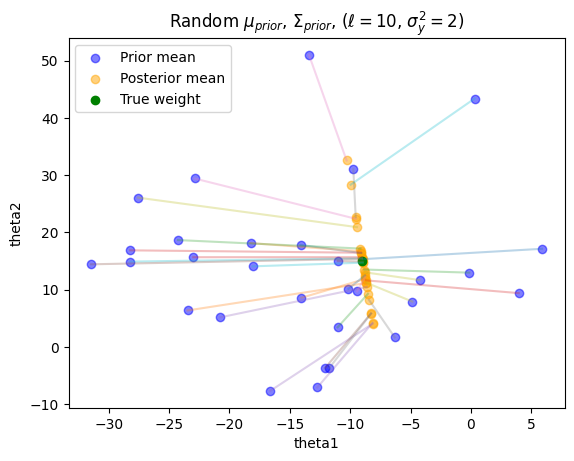
\includegraphics[width=1\textwidth]{assets/week1/random-priors-new-few.png}
\end{subfigure}\\
\begin{subfigure}{.5\textwidth}
  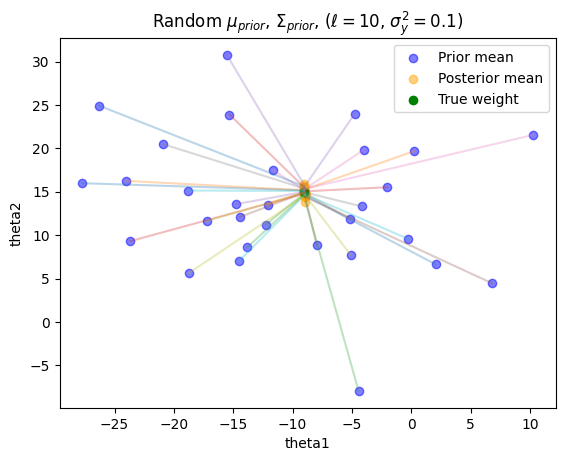
\includegraphics[width=1\textwidth]{assets/week1/random-priors-new-few-accurate.png}
\end{subfigure}%
\begin{subfigure}{.5\textwidth}
  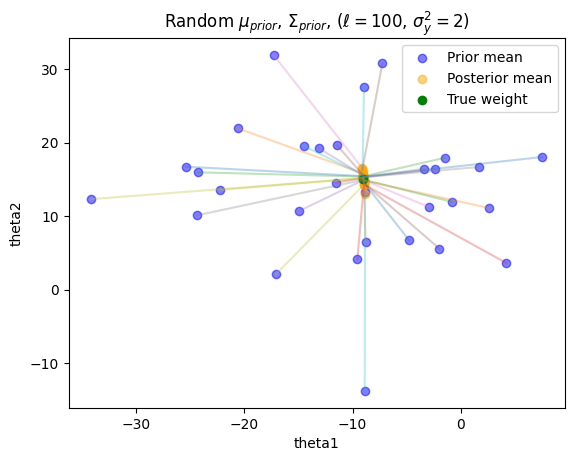
\includegraphics[width=1\textwidth]{assets/week1/random-priors-new-many-inaccurate.png}
\end{subfigure}
\caption{30 different models trained on data sets with different sizes and noise levels. The more samples or lower noise, the closer to the true weights are the posteriors.}
\label{fig:random-prior}
\end{figure}

\begin{figure}[H]
\centering
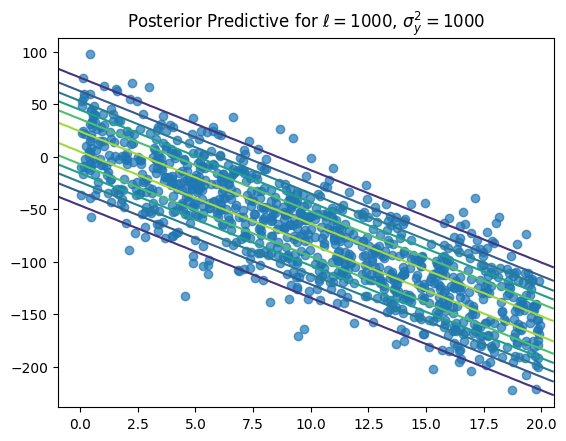
\includegraphics[width=.7\textwidth]{assets/week1/noise-1000.png}
\caption{Contour plot of the posterior predictive distribution.}
\label{fig:posterior-predictive}
\end{figure}
